\section{Grupper}
Gruppeteori er studiet af algebraiske strukturer kendt ved \textit{grupper}. Man kan tænke på en gruppe som et objekt i programmering. Vi kan opstille en masse operationer på dette \textit{objekt}. Især indenfor datalogi er grupper ofte anvendt, da det oftest er nemt at konvertere mellem grupper og kode. I følgende afsnit kigges der først på definitionen for en abelsk gruppe, hvorefter gruppeoperationer på elliptiske kurver bliver defineret både geometrisk og algebraisk.
Vi opskriver definitionen for en \textit{(abelsk)} gruppe (\cite{michaelknudsen2005}). Bemærk at $\oplus$ er en \textit{defineret} operator på $G$. Normalt anvendes et $+$ som notation, men for at adskille det ift andre beregninger bruger jeg $\oplus$.

\begin{mdframed}[frametitle={Definition for en abelsk gruppe}]
En mængde $G$ med en sammensætning $\oplus$ kaldes en gruppe hvis følgende punkter er opfyldt:
\begin{enumerate}\label{tab:definition_af_gruppe}
    \item Lukkethed: For alle $a, b, c \in G$ er $a\oplus b \oplus c\in G$.
    \item Nulelement: Der findes et element $0_{G} \in G$, så $0_{G}\oplus a=a \oplus 0_{G}=a$ for alle $a \in G$.
    \item Invertering: For alle $a\in G$ findes et element $(-a)\in G$ hvor $a\oplus (-a)=0_{G}$.
    \item Associativitet: For alle $a,b,c \in G$ er $a\oplus (b \oplus c)=(a \oplus b)\oplus c$.
    \item Kummutativitet: For alle $a,b,c \in G$ er $a\oplus b \oplus c= c \oplus b \oplus a$.
\end{enumerate}
\end{mdframed}


\subsection{Geometriske Operationer på $E$}
Vi betegner punkter på E med store bogstaver f.eks. $P, Q, -R$ hvor $P \oplus Q=-R$ er det punkt på $E$ vi kommer frem til ved at ”lægge” punkterne $P$ og $Q$ sammen. Som tidligere vist, kan en kurve maksimalt have tre skæringspunkter for en sekantlinje på $E$. Ideen er nu at definere de tre skæringspunkter for en ret linje med kurven $E$ til at deres sum giver nul altså $P \oplus Q \oplus R=0$. Dog for at dette kan være en gruppe kræver det at \textit{”nul”} også er et punkt på $E$ da gruppen skal være lukket. Vi indfører derfor et nulelement kaldet $\mathcal{O}$ som defineres til at være et punkt uendeligt langt væk. Dette nulelement $\mathcal{O}$ vil skære med alle rette skæringslinjer. Der laves følgende figur for bedre at kunne se hvad der sker.

\begin{figure}[H]
    \centering
    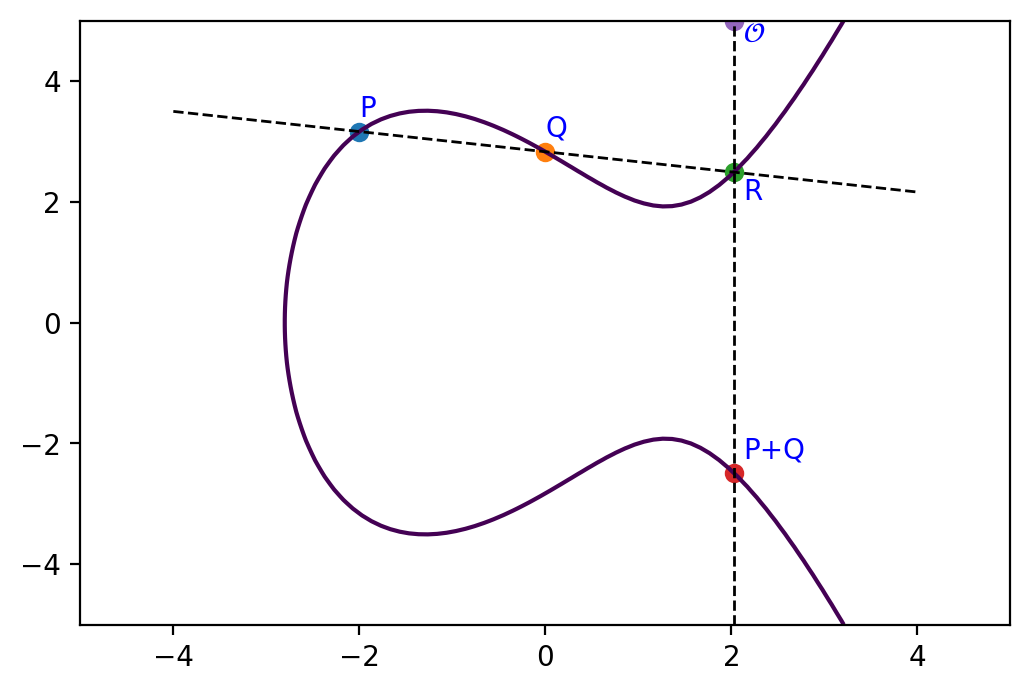
\includegraphics[width=.6\linewidth]{punktaddition.png}
    \caption{Punktaddition på $E$ se \ref{section:figur_2} for kode}
    \label{fig:geo_addition}
\end{figure}


Hvis vi kigger på \fref{fig:geo_addition} er punkterne $P, Q$ samt skæringspunktet $R$ indtegnet. Det inverse element af $R$ svarer til punktet symmetrisk om x-aksen. Vi har altså defineret følgende:
\begin{itemize}
	\item Elementerne for gruppen er punkter på den elliptiske kurve.
	\item Nulelementet er et punkt uendeligt langt væk: $\mathcal{O}$.
	\item Det inverse element for et punkt P er det som er symmetrisk om x-aksen.
	\item Addition er givet ved følgende regel. Givet tre skæringspunkter for en ret linje på en elliptisk kurve, da er deres sum lig med $P\oplus Q \oplus R=\mathcal{O}$.
\end{itemize}

Additionen af punkterne $P$ og $Q$ på \fref{fig:geo_addition} giver altså det inverse punkt af $R$ nemlig $-R$. Der er dog stadigvæk nogle tilfælde som der skal kigges på.

\begin{itemize}
    \item Hvad hvis $P=-Q$? I det her tilfælde vil sekantlinjen gennem de to punkter være vertikal og hermed ikke skære $E$ en tredje gang. Men hvis $P$ er den inverse af $Q$ har vi at. $P \oplus Q=Q \oplus (-Q)=\mathcal{O}$ fra definitionen om invertering se def. \ref{tab:definition_af_gruppe}.
    \item Hvad hvis punktet $Q=P$? Hvis $Q$ går mod $P$ har vi ikke længere en sekantlinje, men en tangent for kurven som vist på \fref{fig:tangent_addition}.
\end{itemize}


\begin{figure}[H]
    \centering
    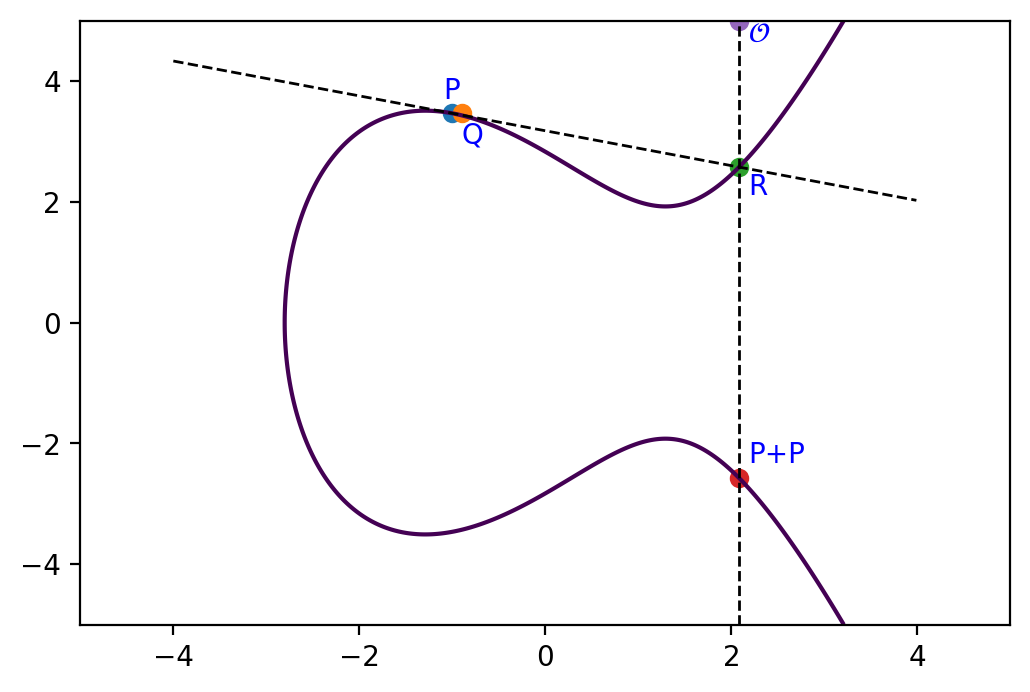
\includegraphics[width=0.7\linewidth]{tangent_addition.png}
    \caption{Punktaddition når $Q$ går mod $P$ se \ref{section:figur_3} for kode}
    \label{fig:tangent_addition}
\end{figure}

Som det kan ses på \fref{fig:tangent_addition} får vi altså at $P\oplus P=-R$ hvor $R$ er det anden skæringspunkt for tangenten.

\subsection{Algebraisk addition}
Hvis vi vil have en computer til at kunne lave overstående addition bliver vi nødt til at finde en algebraisk metode til at lægge punkterne sammen. Dette er også nødvendigt for at vise at definitionen for additionsformler på $E$ gælder (\cite{williamstein2006}) 

\begin{mdframed}[frametitle={Definition for additionsformler på $E$}]
Lad $P, Q$ være punkter på $E$ \fref{eq:ecc}. Det inverse element til $P$ er givet ved:
\begin{equation}\label{eq:invers}
    -P = (x_{P}, -y_{P})
\end{equation}
Ellers udføres additionen $P\oplus Q$ ved at beregne -R.

\begin{equation}
    a=
    \left\{\begin{matrix}\label{eq:slope}
     \frac{y_{P}-y_{Q}}{x_{P}-x_{Q}}& x_{Q} \neq x_P\\\\ 
     \frac{3x_{P}^2+A}{2\cdot y_{P}}& x_P = x_Q
    \end{matrix}\right.
\end{equation}

\begin{equation}
    x=a^2- x_P - x_Q
\end{equation}
\begin{equation}
    y=-a(x - x_P )- y_P
\end{equation}
\begin{equation}
    -R = (x, y)
\end{equation}


\end{mdframed}
Vi udleder nu definitionen for additionsformler på $E$. Vi ved at en ret linje er givet ved:
\begin{equation}\label{eq:ret_linje}
    L: \quad y=ax+b
\end{equation}
Samt ved vi at:
\begin{equation}\label{eq:ret_ligning}
    y = a(x-x_0)+y_0
\end{equation}
Når vi kender koordinaterne for punkterne $P$ og $Q$, kan vi finde hældningen og konstanten for den rette linje gennem punkterne ved:
\begin{equation}
    a = \frac{y_P-y_Q}{x_P-x_Q} \quad x_q \neq x_P
\end{equation}

\begin{equation}\label{eq:constant}
    b=y_P-a \cdot x_P=y_Q -a \cdot x_Q
\end{equation}

Skæringspunkterne mellem L: \fref{eq:ret_linje} og $E$ \fref{eq:E} må være givet ved løsningerne til ligningen:
\begin{equation}
    (ax+b)^2=x^3+Ax+B
\end{equation}

Indsætter \fref{eq:constant}.
$$(ax+y_P-a \cdot x_P )^2=x^3+Ax+B$$
$$(a(x - x_P ) + y_P )^2 = x^3 + Ax + B$$
$$a^2(x^2 + x_{P}^2 - 2x\cdot x_P ) + y_{P}^2 + 2axy_{P} - 2ay_{P}x_P = x^3 + Ax + B$$
\begin{equation}\label{eq:poly}
    \boldsymbol{-a^2} \cdot x_p^2 + 2\cdot a(ax+y_P)\cdot x_P + x^3 + Ax + ax^2 -2axy_P -y_p^2+B=0
\end{equation}
At finde en løsning til en tredjegradsligning kan være meget svært, men da vi kender to rødder ud af tre, kan vi bruge Vieta’s formel (\cite{youssefelhousni2018}).

\begin{mdframed}[frametitle={Vietas formel}]
Lad $P(x)=a_{n}x^n + a_{n-1}x^{n-1}+...+a_{1}x^1+ a_0$ være et polynomie af graden $n$ hvor $a_n \neq 0$. Der gælder da følgende sammenhæng mellem rødderne og koefficienterne:
\begin{equation}\label{eq:vietas}
    x_1 + x_2 + ... +x_n = \frac{-a_{n-1}}{a_n}
\end{equation}
\end{mdframed}

Vi ved at \fref{eq:poly} har tre rødder givet ved $x_P, x_Q$ samt $x_R$. Vi antager nu at roden vi gerne vil finde er $x_{R}$. Vi aflæser nu koefficienten til $x_{P}^2$ til at være $-a^2$. Hermed kan vi opskrive følgende.
$$ x_P + x_Q+x_R = \frac{-(-a^2)}{1} = a^2$$
$$ x_R = a^2- x_P - x_Q$$

Herefter får vi med ligningen for en ret linje \fref{eq:ret_ligning} at:
$$ y_R = a(x_{R}-x_{P})+y_{P} $$
Da $P\oplus Q=-R$ og vi ved at $-R$ er symmetrisk om x-aksen, må det svare til at gange y-koordinatet med $-1$.
\begin{equation}
    -R(x,y)=R(x,-y)
\end{equation}
Operationen for $P\oplus Q$ hvor $P \neq Q$ og punkterne er ikke symmetriske om x-aksen bliver da.
\begin{equation}
    x = a^2 -x_P -x_Q 
\end{equation}
\begin{equation}
    y = -a(x-x_P)-y_p
\end{equation}
\begin{equation}
    P\oplus Q=-R=(x, y)
\end{equation}

Hvor $a$ findes ved \fref{eq:slope}. Vi får dog et problem ved at finde hældningen med \fref{eq:slope} når $P=Q$. Som vi så tidligere gav dette tangenten til kurven $E$. Vi differentierer hermed $E$ ved brug af kædereglen.
$$f(x) = y = \pm \sqrt{x^3 + Ax +B}$$
$$ f'(x) = \pm \frac{3x^2 +A}{2\cdot \sqrt{x^3+Ax+B}}=\pm \frac{3x^2 +A}{2\cdot y}$$
Vi kigger kun på den positive løsning. Vi indsætter x-koordinatet for $P$ eller $Q$, finder vi hældningen $a$ når $x_P=x_Q$
\begin{equation}
    a = f'(x_Q)=f'(x_P)= \frac{3x_{P}^2 +A}{2\cdot y_P} \quad x_P \neq x_Q
\end{equation}

Vi dog stadigvæk anvende de samme formler for at finde $(x, y)$ som anvendt når $x_P \neq x_Q$. Hermed kommer vi frem til definitionen fra forrige afsnit og har hermed vist hvordan formlerne udledes. Det ses også at vi altid får et nyt punkt $-R$ som er en del af den elliptiske kurve da den altid er et skæringspunkt, hvilket gør at vores gruppe er lukket. 

\subsection{Associativitet}
Det eneste vi mangler for at have vist at vores gruppe overholder kriterierne for en gruppe er at den er assosicativ altså $a\oplus(b\oplus c)=(a\oplus b)\oplus c$. Der er et bevis for associativiteten for en gruppe på en elliptisk kurve, men da det mest simple bevis jeg var i stand til at finde fylder ca. 9 sider og bliver betegnet som \textit{"rather messy"} undlader jeg at gennemgå dette. Se (\cite{stefanfriedel2017}) for bevis. I stedet prøver jeg at komme med et logisk argument. 
Hvis vi har punkterne $P,Q,R$ som alle ligger på en ret linje ved vi, at deres orden er ligegyldig betydende, at hvis to punkter går igennem den linje vi laver vil det tredje punkt også. Dette  betyder at hvis alle punkter ligger på en ret linje, må $P\oplus (Q\oplus R)=Q\oplus (P\oplus R)=...=\mathcal{O}$. 

\section{Skalarmultiplikation}
I følgende afsnit introduceres begrebet \textit{skalarmultiplikation}. Udover at kunne lægge punkter sammen en af gangen, opstiller vi en operation til at kunne ligge et punkt \textit{n gange} til sig selv. Vi bruger skalarmultiplikation givet ved:
\begin{equation}
    n \cdot P =\underbrace{P\oplus P\oplus P\oplus ...\oplus P}_\text{n gange}
\end{equation}
Ligesom tidligere som for $\oplus$ er gangetegnet altså ikke en \textit{normal} operation, men i stedet en vi definerer.
Når man kigger på overstående tænkes det at $n \cdot P$ kræver $n$ additioner af punkter altså $O(n)$ i tidskompleksitet. Dette bliver meget hurtigt rigtigt langsomt når $n$ bliver stort Vi kan dog bruge en algoritme som hedder \code{double-and-add} (\cite{andreacorbellini2015}). Vi sætter $n=151$ som eksempel, der ved binær er givet ved $10010111_2$:
$$151=2^7+2^4+2^2+2^1+2^0$$
Hvilket giver:
$$151\cdot P=2^7 \cdot P \oplus 2^4 \cdot P \oplus 2^2 \cdot P \oplus 2^1 \cdot P \oplus 2^0 \cdot P$$
Måden dette udregnes på er så ved at kigge på det binære tal og gå iterativt igennem bits'ne i det. Hvis det enkelte bit er lig med $1$ laver man en addition efterfulgt af en dublering. Hvis det enkelte bit i stedet er lig med $0$ laves der kun en dublering. For overstående får vi altså:
\begin{itemize}
    \item Tag $P$
    \item Dubler $P$ og få $(2\cdot P)$
    \item Lig $2\cdot P$ til $P$
    \item Dubler $2\cdot P$ og få $(2^2 \cdot P)$
    \item osv...
\end{itemize}
Ved brug af overstående metode kan vi udregne $151 \cdot P$ ved bare $7$ dubleringer og $4$ additioner. I implementeringen kan pseudokoden for algoritmen ses i \fref{sec:skalarmultiplikation}, mens koden kan findes i bilaget se \fref{sec:code}. Det vigtigste at tage med er dog at vi i stedet for $O(n)$ reducerer tidskompleksiteten til $O(log_2 n)$, da algoritmen er "lineær" i forhold til længden af det binære tal.


